\documentclass[]{tufte-book}

% ams
\usepackage{amssymb,amsmath}

\usepackage{ifxetex,ifluatex}
\usepackage{fixltx2e} % provides \textsubscript
\ifnum 0\ifxetex 1\fi\ifluatex 1\fi=0 % if pdftex
  \usepackage[T1]{fontenc}
  \usepackage[utf8]{inputenc}
\else % if luatex or xelatex
  \makeatletter
  \@ifpackageloaded{fontspec}{}{\usepackage{fontspec}}
  \makeatother
  \defaultfontfeatures{Ligatures=TeX,Scale=MatchLowercase}
  \makeatletter
  \@ifpackageloaded{soul}{
     \renewcommand\allcapsspacing[1]{{\addfontfeature{LetterSpace=15}#1}}
     \renewcommand\smallcapsspacing[1]{{\addfontfeature{LetterSpace=10}#1}}
   }{}
  \makeatother

\fi

% graphix
\usepackage{graphicx}
\setkeys{Gin}{width=\linewidth,totalheight=\textheight,keepaspectratio}

% booktabs
\usepackage{booktabs}

% url
\usepackage{url}

% hyperref
\usepackage{hyperref}

% units.
\usepackage{units}


\setcounter{secnumdepth}{2}

% citations
\usepackage{natbib}
\bibliographystyle{apalike}

% pandoc syntax highlighting
\usepackage{color}
\usepackage{fancyvrb}
\newcommand{\VerbBar}{|}
\newcommand{\VERB}{\Verb[commandchars=\\\{\}]}
\DefineVerbatimEnvironment{Highlighting}{Verbatim}{commandchars=\\\{\}}
% Add ',fontsize=\small' for more characters per line
\newenvironment{Shaded}{}{}
\newcommand{\AlertTok}[1]{\textcolor[rgb]{1.00,0.00,0.00}{\textbf{#1}}}
\newcommand{\AnnotationTok}[1]{\textcolor[rgb]{0.38,0.63,0.69}{\textbf{\textit{#1}}}}
\newcommand{\AttributeTok}[1]{\textcolor[rgb]{0.49,0.56,0.16}{#1}}
\newcommand{\BaseNTok}[1]{\textcolor[rgb]{0.25,0.63,0.44}{#1}}
\newcommand{\BuiltInTok}[1]{#1}
\newcommand{\CharTok}[1]{\textcolor[rgb]{0.25,0.44,0.63}{#1}}
\newcommand{\CommentTok}[1]{\textcolor[rgb]{0.38,0.63,0.69}{\textit{#1}}}
\newcommand{\CommentVarTok}[1]{\textcolor[rgb]{0.38,0.63,0.69}{\textbf{\textit{#1}}}}
\newcommand{\ConstantTok}[1]{\textcolor[rgb]{0.53,0.00,0.00}{#1}}
\newcommand{\ControlFlowTok}[1]{\textcolor[rgb]{0.00,0.44,0.13}{\textbf{#1}}}
\newcommand{\DataTypeTok}[1]{\textcolor[rgb]{0.56,0.13,0.00}{#1}}
\newcommand{\DecValTok}[1]{\textcolor[rgb]{0.25,0.63,0.44}{#1}}
\newcommand{\DocumentationTok}[1]{\textcolor[rgb]{0.73,0.13,0.13}{\textit{#1}}}
\newcommand{\ErrorTok}[1]{\textcolor[rgb]{1.00,0.00,0.00}{\textbf{#1}}}
\newcommand{\ExtensionTok}[1]{#1}
\newcommand{\FloatTok}[1]{\textcolor[rgb]{0.25,0.63,0.44}{#1}}
\newcommand{\FunctionTok}[1]{\textcolor[rgb]{0.02,0.16,0.49}{#1}}
\newcommand{\ImportTok}[1]{#1}
\newcommand{\InformationTok}[1]{\textcolor[rgb]{0.38,0.63,0.69}{\textbf{\textit{#1}}}}
\newcommand{\KeywordTok}[1]{\textcolor[rgb]{0.00,0.44,0.13}{\textbf{#1}}}
\newcommand{\NormalTok}[1]{#1}
\newcommand{\OperatorTok}[1]{\textcolor[rgb]{0.40,0.40,0.40}{#1}}
\newcommand{\OtherTok}[1]{\textcolor[rgb]{0.00,0.44,0.13}{#1}}
\newcommand{\PreprocessorTok}[1]{\textcolor[rgb]{0.74,0.48,0.00}{#1}}
\newcommand{\RegionMarkerTok}[1]{#1}
\newcommand{\SpecialCharTok}[1]{\textcolor[rgb]{0.25,0.44,0.63}{#1}}
\newcommand{\SpecialStringTok}[1]{\textcolor[rgb]{0.73,0.40,0.53}{#1}}
\newcommand{\StringTok}[1]{\textcolor[rgb]{0.25,0.44,0.63}{#1}}
\newcommand{\VariableTok}[1]{\textcolor[rgb]{0.10,0.09,0.49}{#1}}
\newcommand{\VerbatimStringTok}[1]{\textcolor[rgb]{0.25,0.44,0.63}{#1}}
\newcommand{\WarningTok}[1]{\textcolor[rgb]{0.38,0.63,0.69}{\textbf{\textit{#1}}}}

% longtable
\usepackage{longtable,booktabs}

% multiplecol
\usepackage{multicol}

% strikeout
\usepackage[normalem]{ulem}

% morefloats
\usepackage{morefloats}


% tightlist macro required by pandoc >= 1.14
\providecommand{\tightlist}{%
  \setlength{\itemsep}{0pt}\setlength{\parskip}{0pt}}

% title / author / date
\title{R for Environmental Health Research}
\author{Brooke Anderson}
\date{April 9, 2019}

\usepackage{booktabs}
\usepackage{amsthm}
\usepackage{fontspec}
    \setmainfont{Gill Sans}
\makeatletter
\def\thm@space@setup{%
  \thm@preskip=8pt plus 2pt minus 4pt
  \thm@postskip=\thm@preskip
}
\makeatother

\begin{document}

\maketitle



{
\setcounter{tocdepth}{1}
\tableofcontents
}

\hypertarget{prerequisites}{%
\chapter{Prerequisites}\label{prerequisites}}

\hypertarget{overview}{%
\subsection{Overview}\label{overview}}

\newthought{Based on requests from } some of the students for this
workshop, I've focused here on a few topics relevant to environmental health
research: organizing projects and tracking them with version control, creating
your own packages, and collecting and processing large datasets relevant to
environmental health research. You can download the slides from the workshop by
\href{https://github.com/geanders/columbia_env_health/raw/master/_workshop_slides/workshop_slides.pdf}{clicking
here}.

There are some additional topics in R that would also be useful for
environmental health researchers that I won't cover here. I would, however,
suggest that you look at the latest on tidyverse functions for cleaning and
visualizing data (the \texttt{dplyr} and \texttt{ggplot2} packages are at the heart of this),
new developments on working with geospatial data with the \texttt{sf} package, creating
interactive graphics with \texttt{htmlwidgets}, and creating reports, blogs, and books
through the \texttt{rmarkdown} framework. In the conclusion to this booklet, I'll
provide some references for learning more about all of these topics.

\hypertarget{set-up}{%
\subsection{Set-up}\label{set-up}}

I am assuming that you already have R and RStudio installed on your computer.
You may want to check that you have a recent version of both, and if not, update
you version before the workshop. Some of the packages and RStudio tools we'll be
using will require newer versions of R and RStudio to work. You can run
\texttt{sessionInfo()} in R to find out the version of R you have installed. Compare
this version to the latest R release version listed at the \textbf{Comprehensive R
Archive Network (CRAN)}\footnote{\textbf{Comprehensive R Archive Network (CRAN).} \ldots{}}

To try out the examples, you will also need a bit more set-up:

\begin{enumerate}
\def\labelenumi{\arabic{enumi}.}
\tightlist
\item
  Download git
\item
  Get a GitHub account
\item
  Install some R packages
\item
  Download example R Project
\end{enumerate}

This section will walk you through each step.

\begin{enumerate}
\def\labelenumi{\arabic{enumi}.}
\tightlist
\item
  Download git
\end{enumerate}

In the workshop, you will learn how to use \textbf{git}.{[}\^{}\textbf{git.} Open-source version control
software \ldots{}{]} To try the examples, you will need to install git to your computer and make
sure that your installation of RStudio can find this software, so you can use git for version
control for R Projects. \ldots{}

\begin{enumerate}
\def\labelenumi{\arabic{enumi}.}
\setcounter{enumi}{1}
\tightlist
\item
  Get a GitHub account
\end{enumerate}

You'll also learn how to share and collaborate on an R Project using \textbf{GitHub}.\footnote{\textbf{GitHub.}
  An online platform for directories tracked with
  the version control software \texttt{git}. This platform has become
  very popular for sharing code projects, as well as collaborating across a team on developing
  code and software. Other online git platforms exist and are used by some researchers,
  including \textbf{GitLab}. Once you've mastered using GitHub, you should be able to easy
  transfer those skills to other platforms like GitLab.} You will need to get a GitHub
account to be able to post repositories on GitHub. \ldots{}

\begin{enumerate}
\def\labelenumi{\arabic{enumi}.}
\setcounter{enumi}{2}
\tightlist
\item
  Install some R packages
\end{enumerate}

This booklet uses a number of R packages beyond base R. To install all the packages that you'll
need, run the following code in your version of R:

\begin{Shaded}
\begin{Highlighting}[]
\KeywordTok{install.packages}\NormalTok{(}\KeywordTok{c}\NormalTok{(}\StringTok{"readr"}\NormalTok{, }\StringTok{"ggplot2"}\NormalTok{, }\StringTok{"forcats"}\NormalTok{, }
    \StringTok{"magrittr"}\NormalTok{, }\StringTok{"dplyr"}\NormalTok{, }\StringTok{"lubridate"}\NormalTok{, }\StringTok{"sf"}\NormalTok{, }\StringTok{"tigris"}\NormalTok{, }
    \StringTok{"DT"}\NormalTok{, }\StringTok{"plotly"}\NormalTok{, }\StringTok{"leaflet"}\NormalTok{, }\StringTok{"flexdashboard"}\NormalTok{, }
    \StringTok{"tidyr"}\NormalTok{, }\StringTok{"stringr"}\NormalTok{))}
\end{Highlighting}
\end{Shaded}

\begin{enumerate}
\def\labelenumi{\arabic{enumi}.}
\setcounter{enumi}{3}
\tightlist
\item
  Download example R Project
\end{enumerate}

I've created a repository on GitHub. You can find this example
repository by \href{https://github.com/geanders/columbia_env_health_examples}{clicking here}. On the
page takes you to, click on the ``Clone or download'' button and then select ``Download ZIP''.

This will download a single zipped file to your computer. When you unzip the file, it will be a
special type of directory, an R Project directory. To open the R Project and start on the
examples, open RStudio, then go to ``File'' -\textgreater{} ``Open Project''. A pop-up window will open to let you
navigate through your files and find an R Project to open. Navigate to the directory you
downloaded, which should be called ``columbia\_env\_health\_examples'' and doubleclick on the file
in this directory called ``columbia\_env\_health\_examples.Rproj''.

This will open the project. In the ``Files'' pane of RStudio, you should see some subdirectories for
``R'' and ``data''. These have the example R code and data, respectively, for you to try the examples
in this booklet. The code in each of the R files should run independently, including the code to
load all required packages. Figure \ref{fig:examplerepo} shows what this package should
look like once you've downloaded and opened it, as well as some of the files in the
project's ``R'' subdirectory.

\begin{figure*}
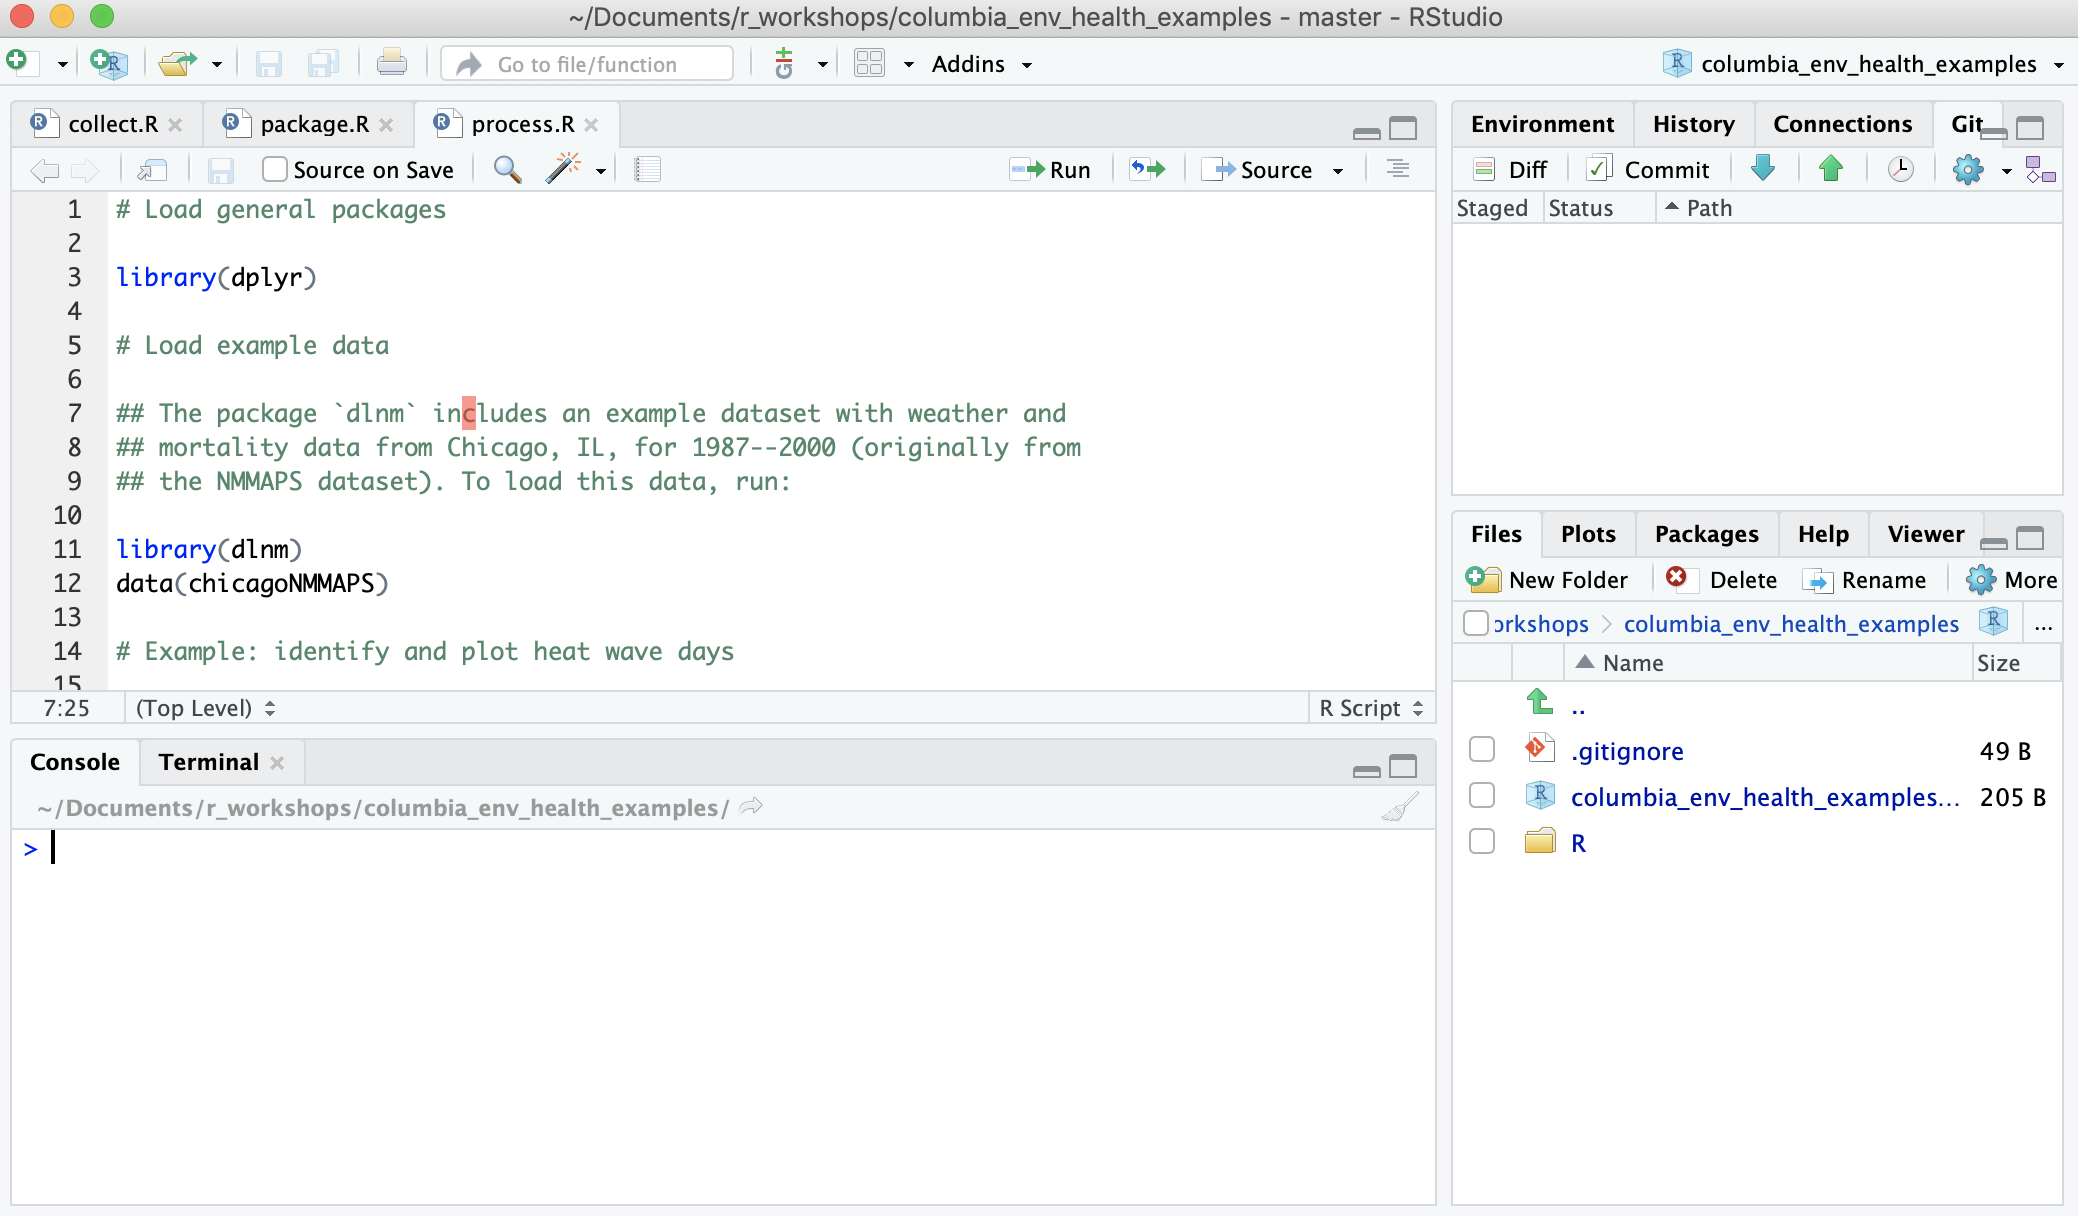
\includegraphics[width=28.86in]{images/example_repo} \caption[What the example R Project for this booklet should look like once you've downloaded and opened it]{What the example R Project for this booklet should look like once you've downloaded and opened it.}\label{fig:examplerepo}
\end{figure*}

Click on the \textbf{Next} button (or navigate using the
links at the top of the page) to continue.

\hypertarget{organize}{%
\chapter{Organize}\label{organize}}

\newthought{If you are using R to write} for larger projects, including research
for academic papers and theses, you should start putting some thought into how you
organize your research files, including raw data, cleaned data, coding scripts for
analysis, and output like paper drafts and figures.

\hypertarget{r-projects}{%
\section{R Projects}\label{r-projects}}

\newthought{RStudio allows you to} create ``Projects'', which help with this
organization. An R Project is very simple---it's just a file directory, with an
extra subdirectory added to the directory {[}with settings?{]}. This directory is
saved as a \textbf{dot file}\footnote{\textbf{dot file.} \ldots{}}, so you probably won't be able to see it
listed if you look at the directory contents using your {[}file viewer?{]}. If you'd like
to see the listing (or delete it by hand, although you likely won't ever need to
do this), check the settings for your {[}file viewer?{]}, and see if you have the option
to show all files. Alternatively, you can use the ``list'' command with the ``all'' option
(\texttt{ls\ -a}) at a Bash shell to view all files and subdirectories in a directory.

Advantages of setting a directory to be an R Project are:

\begin{itemize}
\tightlist
\item
  Automatically uses the directory as your current working directory when you open the project.
\item
  Coordinates well with git version control and GitHub repository system.
\item
  Opens a ``Files'' window for navigating project files in an RStudio pane when you open the project.
\end{itemize}

You can either create an R Project as a new directory or convert an existing directory into
an R Project. To do either, in RStudio go to the ``File'' menu and select ``New Project''. You'll
then have the option to either create a new directory that's an R Project or to search through
your computer's files to find an existing directory to make into an R Project.

Once you've created an R Project, you can open it in RStudio; opening an R Project will set
the project's directory as your working directory, opening a ``Files'' window with all the
subdirectories and files in the project directory and allowing you to run code with
\textbf{relative filenames}\footnote{\textbf{relative filename.} \ldots{}} from the project's directory. If you
share the R Project with someone else,\footnote{One way to do this would be to zipped the directory
  into a single file and share it by email. Another is to use git version control, post the
  directory to GitHub, and share the directory from there.} he or she will also be able to
open the R project using RStudio.

One benefit of R Projects is that it is very easy to initialize them as git repositories.
A later section (``Track'') will go over how to initialize and use git version control for
R Projects. You will also definitely want to use an R Project for any R package you write,
as this will introduce a lot of functionality that ``plays well'' with the \texttt{devtools} package
to make it easier to write, build, and publish an R package {[}?{]}.

\hypertarget{directory-organization}{%
\section{Directory organization}\label{directory-organization}}

\ldots{}

\hypertarget{keeping-things-tidy}{%
\subsection{Keeping things tidy}\label{keeping-things-tidy}}

My desk at work is very messy, with lots of paper printouts piled up. My car and my closet
aren't terribly tidy, either. But I do keep my project directories very tidy, and I
strongly recommend the practice.

This goes beyond ``well-organized'', which we just covered (putting all project
files in one directory, using subdirectories to divide up files in a project,
using consistent names for project file directories, etc.). Keeping a project directory
``tidy'' means having \textbf{only one} version of each file. Often, as you develop a project,
especially when collaborators are involved, you can end up with many versions of a
file. For example, you may have the draft of a journal article's text saved
in some versions with the file name reflecting the date of the draft (``draft\_may\_12.docx''),
some versions that include the initials of people who reviewed it (``paper\_draft\_ba\_rp\_mb2.docx''),
and so on.

This type of organization---having multiple versions of project files, with the file names
meant to help you keep track of them---results in very cluttered and hard-to-manage project
directories. Instead, at any given moment, each of your project directories should have only
one version of each project file. You certainly won't want to lose information from edits
and changes to the files along the way, so it's smart to use some type of \textbf{version control
system}{[}\textbf{version control system.} \ldots{}{]} on each project directory. This will allow you
to track the changes you've made to each file and to go back and revisit the file at any
moment in the project's history. A later section of this booklet will describe how you can
use \texttt{git} for version control for R projects.

\hypertarget{avoiding-repetition}{%
\subsection{Avoiding repetition}\label{avoiding-repetition}}

One key to efficient organization is to \textbf{avoid repetition}.\footnote{In programming, you'll often
  hear this advice as ``Do Not Repeat Yourself''.} In practice, it often happens that you're using the
same code across several projects. For example, say you have some code that calculates the
apparent temperature from air temperature and some measure of dewpoint temperature. If you have
organized your project files to have one directory per paper, with all the associated code for
a paper within the project's directory, then you may find you're often copying and pasting the
code to calculate apparent temperature into different directories.

This situation makes for a tricky balance---you want to organize your files and have a separate
directory for each project, but cutting and pasting code can be a recide for disaster. Each time
you move the code, there's a chance for an error to slip in. Also, what if you want to make a change
in the code? Say you hear about a better algorithm for calculating apparent temperature?
You will either need to go through all of your projects that use that code and change the code
everywhere, or you will have to settle for different projects using different algorithms.

This means it's time to start thinking about writing your own \textbf{R package}.{[}\citet{*}*R package** \ldots{}{]}
You do not have to publish every R package you write---it's fine to just use it yourself and not
share it more widely. Regardless, a package is the right place to store related code that you use
often, as well as documentation (and possibly tests) to go with that code. A later section of this
booklet will go over a bit about how to write your own R packages, as well as references for
learning more about package development.

\hypertarget{learn-more}{%
\section{Learn more}\label{learn-more}}

{[}R Reproc. Research{]} is an excellent book with advice on improving the reproducibility of
projects using R, including academic research projects.

A few good articles have come out recently that describe project organization within
the scientific fields of {[}biology{]} and {[}archaeology{]}. {[}One has links to example repositories?{]}\\
Other papers discuss project organization in the context of reproducibility, presenting
the idea of creating a \textbf{research compendium}\footnote{\textbf{research compendium.} \ldots{}} for scientific
publications.

\hypertarget{track}{%
\chapter{Track}\label{track}}

\newthought{Years ago, I tried to learn to use} git version control software with R, and
it was a total fail. Maybe it's just me, but I found it really hard to wrap my head around
the text-dominated, command-line interface classically used for git. However, RStudio now
includes tools that provide a \textbf{GUI}-style\footnote{\textbf{Graphical User Interface (GUI).} \ldots{}}
interface to most of the functionality you'll need from git for R-based projects. I highly
recommend trying git by using it through RStudio first, and then once you develop a mental
map of what's going on, it's much easier to transfer partially or completely to running git
from a shell.

In this part, I'll discuss both git (the software that allows you to track changes to your
R projects), as well as GitHub (an online platform for sharing and collaborating on
version-controlled projects). I'll also discuss, near the end, how to use either a Bash
Shell or the \texttt{git2r} package to do some one-off git tasks that can't be done directly through
the RStudio GUI-style git interface.

\hypertarget{git}{%
\section{git}\label{git}}

\hypertarget{github}{%
\section{GitHub}\label{github}}

\hypertarget{terminal}{%
\section{Terminal}\label{terminal}}

I find that, for 90\% of what I want to do in git, I can do it through the GUI-style
interface RStudio provides for git. The few exceptions include:

\begin{itemize}
\tightlist
\item
  Setting a remote and doing the initial push to that remote
\item
  Reverting a commit
\item
  Creating a new branch
\item
  Merging two branches
\end{itemize}

For these tasks, I usually open up a \textbf{Bash Shell}\footnote{\textbf{Bash Shell.} A \ldots{} . ``Bash'' stands
  for ``Bourne-Again Shell'', Stephen Bourne, a Unix developer.} and run a git command from
there. However, there's also a package called \texttt{git2r} that lets you run any of these
git commands from the R command line, so you could also do all these (fairly rare) tasks
from the R console without ever opening a Bash Shell, if you master the \texttt{git2r} package.

\hypertarget{accessing-a-bash-shell}{%
\subsection{Accessing a Bash Shell}\label{accessing-a-bash-shell}}

\hypertarget{git2r-package}{%
\subsection{\texorpdfstring{\texttt{git2r} package}{git2r package}}\label{git2r-package}}

\hypertarget{learn-more-1}{%
\section{Learn more}\label{learn-more-1}}

Hadley Wickham's excellent book on \href{http://r-pkgs.had.co.nz/}{R Packages} includes a great
chapter on \href{http://r-pkgs.had.co.nz/git.html}{Git and GitHub}. While the chapter (and book) is
focused on R packages specifically, the guidance in this chapter would apply to any
R Project directory under version control, whether or not the R Project is for a package.
This book is available free online or as a print version through O'Reilly (and
carried at many Barnes \& Nobles).

If you're using git a lot for R projects, it's helpful to have some resources available with
more on using git through a Bash Shell. I like the book \href{https://www.amazon.com/Pragmatic-Guide-Git-Programmers/dp/1934356727/ref=sr_1_28?keywords=git\&qid=1554173700\&s=gateway\&sr=8-28}{Pragmatic Guide to Git} by Travis Swicegood for a quick, short reference and
\href{https://www.amazon.com/Git-Practice-Techniques-Mike-McQuaid/dp/1617291978/ref=sr_1_60?keywords=git\&qid=1554174811\&s=gateway\&sr=8-60}{Git in Practice} by Mike McQuaid if I'm trying to dig a bit deeper
and figure out how git works.
I have also heard good things about \href{https://git-scm.com/book/en/v2}{Pro Git} by Scott Chacon and
Ben Straub, which is available for free online.

However, these resources are all geared to those using git for its original purpose of
tracking changes in software development projects. When you use git to track files for a research
project (rather than, for example, for a repository for an R package you're writing), you
may have some needs that don't come up under software development. A few articles have come
out recently that give advice on using git specifically to track research projects---these provide
helpful advice specific to this use of git, which you won't find in books about git.

\href{https://stackoverflow.com/}{\textbf{StackOverflow}}\footnote{\href{https://stackoverflow.com/}{\textbf{StackOverflow}}.
  \ldots{}}
is also invaluable to quickly look up how to do something in git. There are
many tasks in git where I never remember the command, but I do remember enough about what
the functionality is called to be able to quickly use Google to find a StackOverflow thread
that gives me the call. Reading through a book or tutorial on git, even if you don't
remember the commands you learn, can help you learn some of the vocabulary\footnote{Some good git-related
  words to know to help you search for calls for rarer tasks: ``commit'', ``branch'', ``merge'', ``revert'',
  ``push'', ``pull'', ``merge conflict'', ``remote'', ``origin'', ``master'', ``fork'', ``clone'', ``pull request''.},
and knowing that vocabulary will help you search for answers when you need them.

Finally, if you can find a way to do it, I think the best and easiest way to learn to use git
and GitHub with R is to collaborate with someone who's used these tools before. Most of the
time, these tools are very easy to use, but the small percent of the time that they're not,
it can be significant stumbling blocks (in terms of the time it takes to figure out the fix)
the first few times you use the tools, while someone familiar with them and working on the
project can diagnose and get you over those bumps as you learn the ropes.

\hypertarget{package}{%
\chapter{Package}\label{package}}

\newthought{As with many other things in R,} the threshold of complexity
for writing your own package has recently lowered dramatically. If you are writing
some of your own functions in R to use for your research, and you've become comfortable
with writing functions, you should try putting them in an R package. You don't have
to share this package through publishing it on CRAN or another repository---instead, it's
fine to start by just writing packages for your own use, or for your research group's
private use. However, once you start writing packages, you will see how straightforward
it is, and you may want to take the extra steps to prepare your package for CRAN and
submit it.

\hypertarget{r-packages}{%
\section{R packages}\label{r-packages}}

\hypertarget{r-code}{%
\subsection{R code}\label{r-code}}

{[}Where to put it{]}

{[}How to add documentation{]}

\hypertarget{description-file}{%
\subsection{DESCRIPTION file}\label{description-file}}

\begin{itemize}
\tightlist
\item
  License
\end{itemize}

\hypertarget{other-package-components}{%
\subsection{Other package components}\label{other-package-components}}

So far, I've described the barebones elements you'll need to have to create a very
minimalist package. There are, however, a number of other elements you'll often
want to add to the package. As with the R code for package functions and the
DESCRIPTION file, there is a specific location and format required for each of
these elements within an R package.

Some of the most common components you'll want to add are:

\begin{itemize}
\tightlist
\item
  \textbf{Example data.}
\item
  \textbf{Vignettes.}
\item
  \textbf{Unit tests.}
\end{itemize}

To help you set up these extra components,
you may want to take a look at the \texttt{use\_*} family of functions in the \texttt{usethis}
\citep{R-usethis}
package\footnote{The \texttt{use\_*} family of functions were previously in the \texttt{devtools} package, but they
  are being deprecated there and moved to the \texttt{usethis}
  package. The \href{http://r-pkgs.had.co.nz/}{R Packages} book was written before they were deprecated
  in \texttt{devtools}, and so it discusses them as \texttt{devtools} functions. As long as you install and load
  the \texttt{usethis} package, though, you'll have no problem following along with the examples in
  that book.} For example, if you want to include example data in your package,
you should check out the \texttt{use\_data} function, while if you want to add unit tests to your
package, check out the \texttt{use\_test} function. When you run one of these, you'll notice that the
function \emph{adds files and subdirectories} when needed to your R package directory. This may
throw you at first, since most R functions don't make changes to your file directory, but
you'll need those added files to add the package components, and it's \emph{much} easier to
remember a single function call to run when you need to add one than to remember all the
details of which files and in what structure need to be added.

\hypertarget{publishing}{%
\section{Publishing}\label{publishing}}

\hypertarget{why-publish-your-packages}{%
\subsection{Why publish your packages?}\label{why-publish-your-packages}}

\hypertarget{where-to-publish-packages}{%
\subsection{Where to publish packages}\label{where-to-publish-packages}}

\hypertarget{extra-steps-for-publishing}{%
\subsection{Extra steps for publishing}\label{extra-steps-for-publishing}}

If you want to submit your package to CRAN, you'll need to take a few extra steps
to get it ready. These steps aren't necessary for a package you plan to just
use privately, but they wouldn't be a bad idea to try to do even in that case.

First, you'll need to make sure that the functions in your package are
comprehensively documented. {[}What are requirements for this for CRAN?{]}

In addition to documenting specific functions, you should also consider
writing overall tutorials that walk a user through how to use your
package in a few example scenarios. \textbf{vignette}\footnote{\textbf{vignette.} \ldots{}}

You will also need to make sure that your package can run on different
operating systems. If your package only has functions written exclusively
in R, and doesn't interact with {[}the computer system?{]} or other programs
on your computer, this shouldn't be an issue. However, you should still
check. {[}Travis CI, winbuilder{]}

{[}CRAN checks{]}

\hypertarget{checking}{%
\section{Checking}\label{checking}}

\hypertarget{try-it-out}{%
\section{Try it out}\label{try-it-out}}

\begin{itemize}
\tightlist
\item
  Create a new R Project for an R package
\item
  Move a function into the right place in the package
\item
  Edit the DESCRIPTION file as needed
\item
  Build the package
\item
  Add example data into the right place in the package
\item
  Add some unit tests for the function
\item
  Add documentation using roxygen2 notation
\item
  Add a short vignette
\end{itemize}

\hypertarget{learn-more-2}{%
\section{Learn more}\label{learn-more-2}}

One wonderful resource for writing and publishing R packages is the book \href{http://r-pkgs.had.co.nz/}{R
Packages} by Hadley Wickham. This book is available
for a reasonable price in paperback (many Barnes \& Nobles carry it in their
computer section) and is also available for free online. The author of this book
also created and maintains the \textbf{\texttt{devtools} package}\footnote{\textbf{\texttt{devtools} package.}
  An R package with functions that facilitate R package development. These
  functions are well-documented in the package documentation as well as through
  the book \href{http://r-pkgs.had.co.nz/}{R Packages}. This package also includes a
  function for installing R packages from code posted on GitHub
  (\texttt{install\_github}), which is very useful if you want to find and use packages
  that are not yet available on CRAN and other repositories or if you want to use
  the latest, ``development'' version of a package. This package is available on
  CRAN and so can be installed with \texttt{install.packages("devtools")}.}

\begin{itemize}
\tightlist
\item
  ROpenSci handbook
\item
  Official R documentation
\item
  Coursera, Leanpub
\end{itemize}

\hypertarget{collect}{%
\chapter{Collect}\label{collect}}

\newthought{For Environmental Health researchers, I think} one of the most exciting
developments in R recently is how it is changing how we can collect data, both for
exposures and outcomes. One direction for this development is how researchers can
collect and measure original data from experiments, including through new measurement
technologies (e.g., phone-based Apps) and through new or rapidly changing health-related
measurements (e.g., metabolomics, flow cytometry) and associated open-source
software.

R is also facilitating and leveraging rapid developments in how researchers can access and
query secondary data, including from {[}large admin databases?{]} and {[}data repositories
encouraged or required for some NIH-funded projects{]}. \ldots{} This section will provide an
introduction to some of the ideas and techniques behind these developments for
collecting secondary or public-use data for environmental health research, as well as
give you somee directions on where to go to find R packages that facilitate collecting
open data from R.

\hypertarget{open-data}{%
\section{Open data}\label{open-data}}

A range of environmental datasets are available online, especially through national agencies.
For example, {[}NOAA{]} provides various weather datasets, while USGS has data on water quality,
{[}others{]}

You can visit webpages hosted by these agencies where you can download the datasets you need.
However, this process can become tedious if you need lots of datasets, as may be the case for
large studies incorporating many cities. Further, downloading the datasets ``by hand'' is hard
to make reproducible, unless you meticiously write down all the steps you took as you visited
the website. This means that your process will be harder for you to repeat in the future
or for others to replicate.

A growing collection of R packages are now available that allow you to download datasets
available online directly from R. This means that you can write an R script for your data
collection, making this step both better documented and more reproducible. \ldots{}

Further, there are now a number of R packages that provide access to open datasets that the
package maintainer collected and processed and is now making available as an R package.
{[}More on R data packages.{]}

\hypertarget{admin-databases}{%
\subsection{{[}Admin databases?{]}}\label{admin-databases}}

Data collected by government groups like EPA, NOAA, USGS.

\hypertarget{research-repositories}{%
\subsection{{[}Research repositories?{]}}\label{research-repositories}}

Here, especially health-related data.
NIH-supported (e.g., Metabolomics Workbench).
NHANES?

\hypertarget{data-packages}{%
\section{Data packages}\label{data-packages}}

\ldots{}

This package is too big for CRAN to host, so we have it posted through our own package
repository.\footnote{For more on how and why we did this, see
  \href{https://journal.r-project.org/archive/2017/RJ-2017-026/}{an article} we wrote about the
  process for \textbf{The R Journal}.} Because of this, you'll need to take a few extra steps
to download and install the package:\footnote{If you don't have the \texttt{drat} package, install it in
  the usual way with \texttt{install.packages("drat")}.}

\begin{Shaded}
\begin{Highlighting}[]
\KeywordTok{library}\NormalTok{(drat)}
\KeywordTok{addRepo}\NormalTok{(}\StringTok{"geanders"}\NormalTok{)}
\KeywordTok{install.packages}\NormalTok{(}\StringTok{"hurricaneexposuredata"}\NormalTok{)}
\KeywordTok{install.packages}\NormalTok{(}\StringTok{"hurricaneexposure"}\NormalTok{)}
\end{Highlighting}
\end{Shaded}

Once you've installed both the \texttt{hurricaneexposuredata} and \texttt{hurricaneexposure} packages, you
can load them as usual to access both the data and some functions to work with them:

\begin{Shaded}
\begin{Highlighting}[]
\KeywordTok{library}\NormalTok{(hurricaneexposuredata)}
\KeywordTok{library}\NormalTok{(hurricaneexposure)}
\end{Highlighting}
\end{Shaded}

The \texttt{hurricaneexposure} package has a series of functions that let you explore different
exposures during storms. For example, to get the storms where either New York County, NY,
or Suffolk County, MA, (which includes Boston) were exposed to tropical storm-level winds
(17.5 m/s or higher), you can run:\footnote{For any of these functions, you can find out what parameters
  to include, and in what format, but opening the helpfile for the function. For example, once you've
  loaded the \texttt{hurricaneexposure} package, you can open the helpfile for the \texttt{county\_wind} function
  by calling \texttt{?county\_wind}. Also helpful for navigating packages: take advantage of the \texttt{package::function}
  notation and RStudio's tab completion to look up the names of functions in a package. For example,
  type \texttt{hurricaneexposure::}. A pop-up window should show up with all the functions in the package (press
  Tab if the pop-up doesn't automatically open).}

\begin{Shaded}
\begin{Highlighting}[]
\NormalTok{knitr}\OperatorTok{::}\KeywordTok{include_graphics}\NormalTok{(}\StringTok{"images/tab_completion_example.png"}\NormalTok{)}
\end{Highlighting}
\end{Shaded}

\begin{marginfigure}
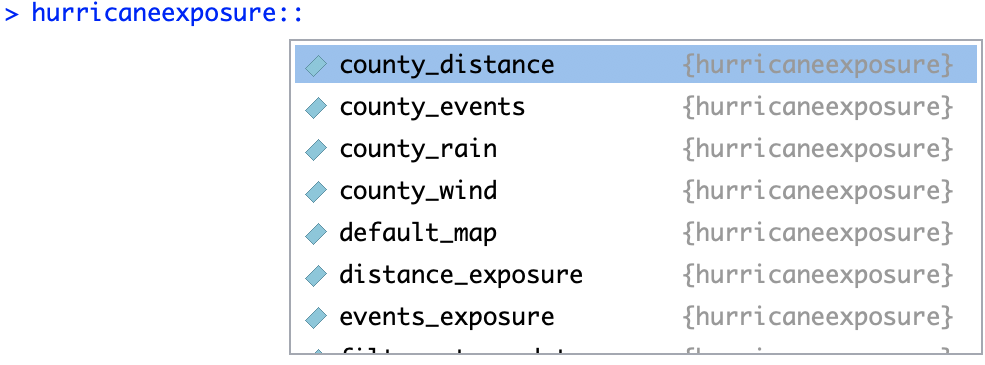
\includegraphics[width=13.68in]{images/tab_completion_example} \end{marginfigure}

\begin{Shaded}
\begin{Highlighting}[]
\KeywordTok{county_wind}\NormalTok{(}\DataTypeTok{counties =} \KeywordTok{c}\NormalTok{(}\StringTok{"36061"}\NormalTok{, }\StringTok{"25025"}\NormalTok{), }\DataTypeTok{start_year =} \DecValTok{1988}\NormalTok{, }
    \DataTypeTok{end_year =} \DecValTok{2015}\NormalTok{, }\DataTypeTok{wind_limit =} \FloatTok{17.5}\NormalTok{)}
\end{Highlighting}
\end{Shaded}

\begin{verbatim}
##       storm_id  fips vmax_sust vmax_gust
## 1     Bob-1991 25025  26.46639  39.43492
## 2     Bob-1991 36061  18.19559  27.11142
## 3  Bertha-1996 25025  29.64453  44.17035
## 4  Bertha-1996 36061  28.95496  43.14289
## 5   Floyd-1999 25025  24.46946  36.45949
## 6   Floyd-1999 36061  20.50178  30.54765
## 7   Hanna-2008 25025  18.36505  27.36392
## 8   Hanna-2008 36061  19.25390  28.68832
## 9   Irene-2011 36061  25.68553  38.27144
## 10  Sandy-2012 36061  21.99213  32.76827
##    sust_dur gust_dur closest_time_utc
## 1       210      570 1991-08-19 20:00
## 2         0      480 1991-08-19 15:00
## 3       240      525 1996-07-14 01:15
## 4       180      540 1996-07-13 19:45
## 5       345      750 1999-09-17 07:45
## 6        60      315 1999-09-17 00:15
## 7         0      150 2008-09-07 07:15
## 8         0      195 2008-09-07 01:45
## 9       165      510 2011-08-28 13:15
## 10      225      795 2012-10-30 00:30
##    storm_dist       local_time closest_date
## 1   27.042565 1991-08-19 16:00   1991-08-19
## 2  161.571830 1991-08-19 11:00   1991-08-19
## 3   38.177990 1996-07-13 21:15   1996-07-13
## 4   16.966013 1996-07-13 15:45   1996-07-13
## 5   51.254726 1999-09-17 03:45   1999-09-17
## 6   45.408483 1999-09-16 20:15   1999-09-16
## 7    6.202866 2008-09-07 03:15   2008-09-07
## 8   29.916672 2008-09-06 21:45   2008-09-06
## 9    5.796733 2011-08-28 09:15   2011-08-28
## 10 158.040788 2012-10-29 20:30   2012-10-29
\end{verbatim}

If you look up events based on flood events, you can instead run the
\texttt{county\_events} function:

\begin{Shaded}
\begin{Highlighting}[]
\KeywordTok{county_events}\NormalTok{(}\DataTypeTok{counties =} \KeywordTok{c}\NormalTok{(}\StringTok{"36061"}\NormalTok{, }\StringTok{"25025"}\NormalTok{), }
    \DataTypeTok{start_year =} \DecValTok{1988}\NormalTok{, }\DataTypeTok{end_year =} \DecValTok{2015}\NormalTok{, }\DataTypeTok{event_type =} \StringTok{"flood"}\NormalTok{)}
\end{Highlighting}
\end{Shaded}

\begin{verbatim}
##     fips     storm_id closest_time_utc
## 1  25025  Dennis-1999 1999-09-08 08:00
## 2  36061   Floyd-1999 1999-09-17 00:15
## 3  36061 Allison-2001 2001-06-17 14:15
## 4  36061 Frances-2004 2004-09-09 13:30
## 5  36061    Ivan-2004 2004-09-18 17:45
## 6  36061  Jeanne-2004 2004-09-29 06:30
## 7  36061   Beryl-2006 2006-07-20 22:15
## 8  36061   Barry-2007 2007-06-04 15:45
## 9  36061   Irene-2011 2011-08-28 13:15
## 10 25025   Sandy-2012 2012-10-29 22:00
## 11 25025  Andrea-2013 2013-06-08 11:30
## 12 36061  Andrea-2013 2013-06-08 06:45
##    storm_dist       local_time closest_date
## 1  390.047523 1999-09-08 04:00   1999-09-08
## 2   45.408483 1999-09-16 20:15   1999-09-16
## 3  158.909890 2001-06-17 10:15   2001-06-17
## 4  379.343696 2004-09-09 09:30   2004-09-09
## 5  311.346881 2004-09-18 13:45   2004-09-18
## 6  222.900157 2004-09-29 02:30   2004-09-29
## 7  207.358443 2006-07-20 18:15   2006-07-20
## 8  148.251718 2007-06-04 11:45   2007-06-04
## 9    5.796733 2011-08-28 09:15   2011-08-28
## 10 433.295980 2012-10-29 18:00   2012-10-29
## 11  45.412565 2013-06-08 07:30   2013-06-08
## 12  92.381282 2013-06-08 02:45   2013-06-08
\end{verbatim}

The \texttt{hurricaneexposure} package also has functions for mapping the exposure
data for specific storms. For example, to see the rainfall fro Hurricane Ivan in
2004, you can run:

\begin{Shaded}
\begin{Highlighting}[]
\KeywordTok{map_counties}\NormalTok{(}\DataTypeTok{storm =} \StringTok{"Ivan-2004"}\NormalTok{, }\DataTypeTok{metric =} \StringTok{"rainfall"}\NormalTok{)}
\end{Highlighting}
\end{Shaded}

\begin{figure*}
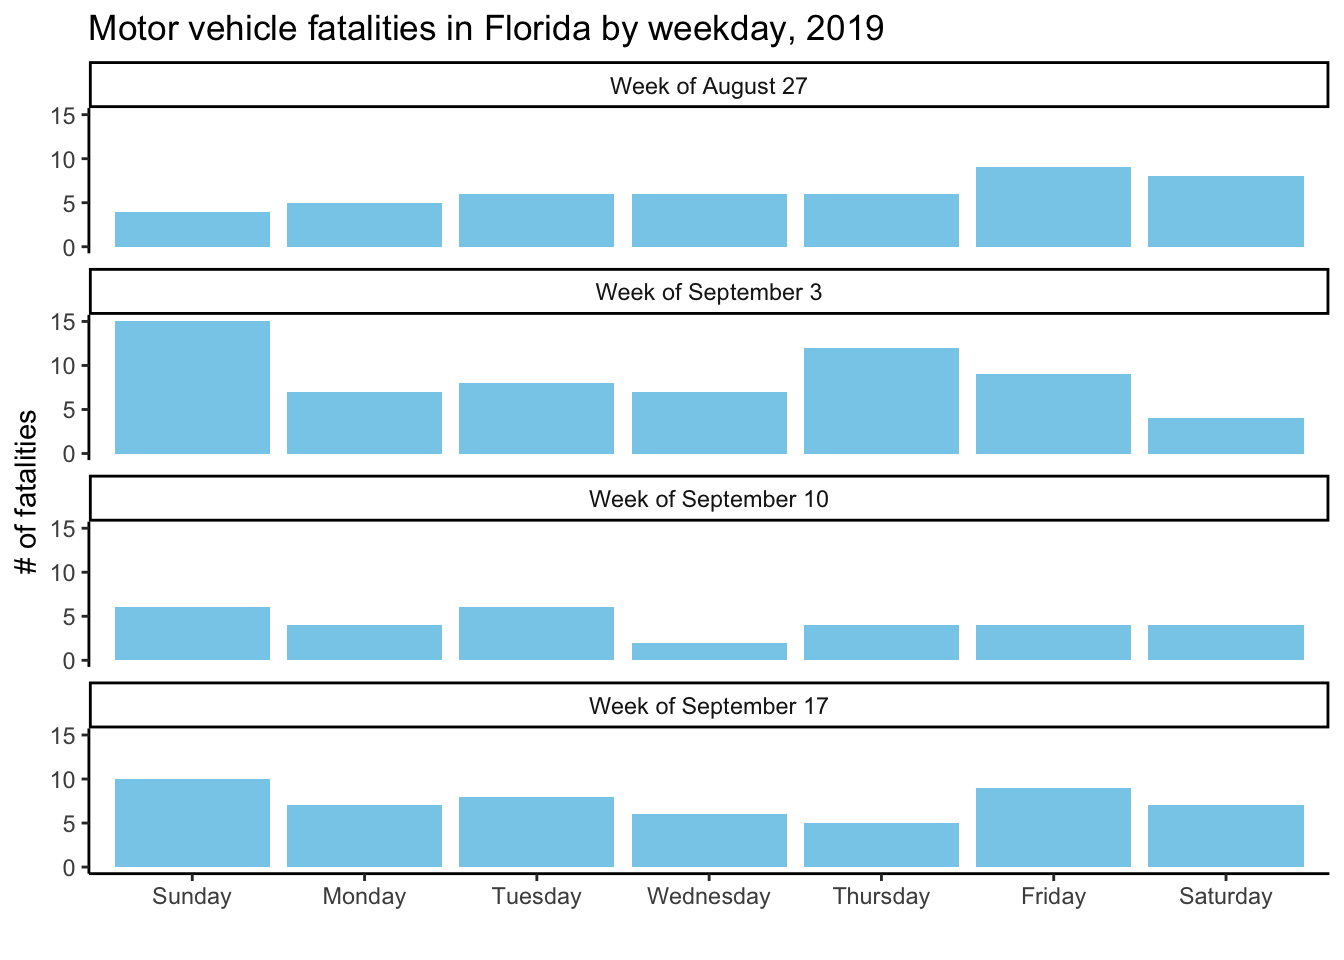
\includegraphics{columbia_env_health_files/figure-latex/unnamed-chunk-9-1} \end{figure*}

From this map, you can see that the rain from this storm extended into New
England, even after the storm looped back around to the east and south. This is
why New York City had heavy rainfall (and flooding) from this event, but not
tropical storm-level winds.

For more on the \texttt{hurricaneexposure} package, see \href{https://cran.r-project.org/web/packages/hurricaneexposure/vignettes/hurricaneexposure.html}{its vignette}

\hypertarget{web-services}{%
\section{Web services {[}?{]}}\label{web-services}}

\hypertarget{ropensci}{%
\section{ROpenSci}\label{ropensci}}

One of the best places to explore R packages for accessing open data for science is
\href{https://ropensci.org/}{\textbf{ROpenSci}}.\footnote{\href{https://ropensci.org/}{\textbf{ROpenSci}}. \ldots{}}
Many of its packages facilitate access to databases of open data relevant to scientific
research that have API access {[}?{]}. You can browse through its packages on
its \href{https://ropensci.org/packages/}{\textbf{Packages} page}

Examples of some packages relevant to collecting data for environmental health research
include:

\begin{itemize}
\tightlist
\item
  bomrang: Australian Government Bureau of Meteorology (`BOM') Data Client
\item
  clifro: Easily Download and Visualise Climate Data from CliFlo
\item
  dbhydroR: `DBHYDRO' Hydrologic and Water Quality Data
\item
  essurvey: Download Data from the European Social Survey on the Fly
\item
  FedData: Functions to Automate Downloading Geospatial Data Available from Several Federated Data Sources
\item
  camsRad: R Client for CAMS Radiation Service
\item
  ccafs: CCAFS GCM Data R Client
\item
  dbhydroR: R interface to the South Florida Water Management District's DBHYDRO Database
\item
  biomartr: Genomic Data Retrieval
\item
  clifro: Easily Download and Visualise Climate Data from CliFlo
\item
  DataSpaceR: An R Interface to `the CAVD DataSpace'
\item
  essurvey: Download Data from the European Social Survey on the Fly
\item
  fingertipsR: Fingertips Data for Public Health
\item
  getCRUCLdata: Use and Explore `CRU' `CL' v. 2.0 Climatology Elements
\item
  getlandsat: Get Landsat 8 Data from Amazon Public Data Sets
\item
  googleLanguageR: Call Google's `Natural Language' API, `Cloud Translation' API, `Cloud Speech'
  API and `Cloud Text-to-Speech' API
\item
  GSODR: Global Surface Summary of the Day (`GSOD') Weather Data Client
\item
  hydroscoper: Interface to the Greek National Data Bank for Hydrometeorological Information
\item
  MODIStsp: A Tool for Automating Download and Preprocessing of MODIS Land Products Data
\item
  nasapower: NASA POWER API Client
\item
  opencage: Interface to the OpenCage API
\item
  osmdata: Import `OpenStreetMap' Data as Simple Features or Spatial Objects
\item
  weathercan: Download Weather Data from the Environment and Climate Change Canada Website
\item
  wateRinfo: Download Time Series Data from Waterinfo.be
\item
  USAboundariesData: Datasets for the `USAboundaries' package
\item
  USAboundaries: Historical and Contemporary Boundaries of the United States of America
\item
  tidyhydat: Extract and Tidy Canadian `Hydrometric' Data
\item
  stats19: Work with Open Road Traffic Casualty Data from Great Britain
\item
  smapr: Acquisition and Processing of NASA Soil Moisture Active-Passive (SMAP) Data
\item
  rWBclimate: A package for accessing World Bank climate data
\item
  rusda: Interface to USDA Databases
\item
  rsnps: Get `SNP' (`Single-Nucleotide' `Polymorphism') Data on the Web
\item
  rrricanesdata: Data for Atlantic and east Pacific tropical cyclones since 1998
\item
  rrricanes: Web scraper for Atlantic and east Pacific hurricanes and tropical storms
\item
  ropenaq: Accesses Air Quality Data from the Open Data Platform OpenAQ
\item
  rnoaa: `NOAA' Weather Data from R
\item
  rnaturalearth: World Map Data from Natural Earth
\item
  riem: Accesses Weather Data from the Iowa Environment Mesonet
\item
  rgpdd: R Interface to the Global Population Dynamics Database
\item
  rdhs: API Client and Dataset Management for the Demographic and Health Survey (DHS) Data
\item
  rdefra: Interact with the UK AIR Pollution Database from DEFRA
\item
  prism: Access Data from the Oregon State Prism Climate Project
\end{itemize}

Cleaning / exploring data:

\begin{itemize}
\tightlist
\item
  cleanEHR: The Critical Care Clinical Data Processing Tools
\item
  colocr: Conduct Co-localization Analysis of Fluorescence Microscopy Images
\item
  cRegulome: Obtain and Visualize Regulome-Gene Expression Correlations in Cancer
\item
  EndoMineR: Functions to mine endoscopic and associated pathology datasets
\item
  geoaxe: Split `Geospatial' Objects into Pieces
\item
  hddtools: Hydrological Data Discovery Tools
\item
  isdparser: Parse `NOAA' Integrated Surface Data Files
\item
  visdat: Preliminary Visualisation of Data
\item
  skimr: A frictionless, pipeable approach to dealing with summary statistics
\end{itemize}

\hypertarget{learn-more-3}{%
\section{Learn more}\label{learn-more-3}}

\begin{itemize}
\tightlist
\item
  ROpenSci
\item
  The R Journal
\item
  CRAN task views?
\item
  ROpenSci articles?
\item
  JOSS?
\end{itemize}

\hypertarget{process}{%
\chapter{Process}\label{process}}

\newthought{For environmental health research,} once you have collected your raw data,
you will often need to do a bit of work processing the data before you can apply epidemiological
models. As one example, you may pull \textbf{gridded data}\footnote{\textbf{gridded data.} \ldots{}} on an
environmental exposure of interest, but need to link it with health data that is aggregated
based on administrative boundaries (e.g., counties). As another example, you might have
daily temperature data and want to identify the dates of heat waves in a community based on
that data.

R has some wonderful tools for processing data that are relevant to environmental health research.
Here, I'll focus on tools from a few packages I've developed, but in ``Learn more'', I'll also
point you to more resources for finding R tools that might be relevant to your own environmental
health research projects.

I strongly encourage you, as you work through this section, to start thinking about possibly
creating your own R packages to solve data processing tasks you commonly face for your research.
All the code for the packages I'll discuss is available on GitHub, so you can look at this code
as examples as you think about writing your own packages.

\hypertarget{learn-more-4}{%
\section{Learn more}\label{learn-more-4}}

\begin{itemize}
\tightlist
\item
  CRAN taskviews
\item
  Bioconductor {[}taskviews?{]}
\item
  ROpenSci
\end{itemize}

{[}CRAN{]} One excellent example of CRAN-based packages {[}?{]} for processing environmental
data is the suite of packages created and maintained by scientists at the \textbf{United States
Geological Survey (USGS)}\footnote{\textbf{United States Geological Survey (USGS).} \ldots{}}
This group has a collection of packages, listed at \ldots{} . The packages include \ldots{}
For a very cool example of using some of these packages for a timely application for
environmental health, check out these visualizations of flooding during Hurricanes \ldots{},
as well as the code used to create them.

For biological data, \textbf{Bioconductor}\footnote{\textbf{Bioconductor.} \ldots{}} can be a great
resource for finding packages to process and pull out relevant data. For example,
Bioconductor has a large collection of packages for working with biological data collected
through flow cytometry, mass spectrometry (e.g., metabolomics), RNA sequencing, {[}others{]}

\hypertarget{final-words}{%
\chapter{Final Words}\label{final-words}}

\bibliography{book.bib,packages.bib}



\end{document}
